\graphicspath{{./figures}}

\section{High-Level System}
There are various decisions to be made regarding the entire communication system. A complete high-level system block diagram illustrating the decisions discussed below is shown in Figure \ref{fig:complete_system}. Note that the yellow blocks are external (i.e. already-provided systems).

\begin{figure}[!htb]
    \centering
    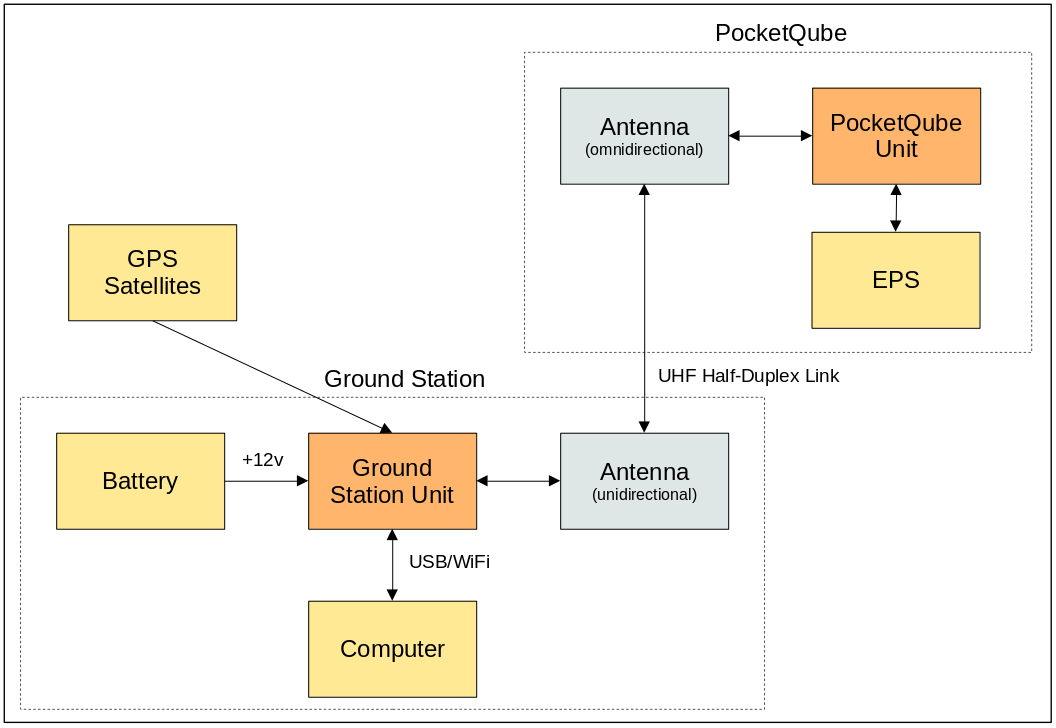
\includegraphics[width=0.8\textwidth]{complete_system.png}
    \caption{Complete High-Level Diagram of Communication System}
    \label{fig:complete_system}
  \end{figure}

\newpage
Firstly, since this project is consists (to a large degree) of system-level design, components integrated into modules (e.g. an "RF module") will be used as much as possible to simplify the integration. Only if no modules are found to meet the system requirements, should a more custom solution be developed.

It is know that open-loop path-predicted tracking is adequate for high-altitude balloons. In this sense, the ground station requires at least a GPS connection, as well as some form of intertial measurement unit (IMU) for beem steering. The path data will be uploaded to the ground station via USB or WiFi and an external device, such as a laptop, personal computer or smartphone (referred to as the system's \textit{computer} onwards). Further, this computer will be used to monitor the link and record the data.

The requirement to communicate with the existing Radiosonde should be considered. According to the iMet54's datasheet \cite{datasheet-iMet54}, it operates at a centre frequency of between 402 and 405 MHz, selected in 1 MHz increments. Ideally, for a simpler design, one antenna should be designed on the GS supporting both the custom and proprietary communication communication protocols.

If very long-range communication is to be supported, a highly-directive antenna will most likely be needed and, as mentioned in Section \ref{sec:antennas}, these antennas are usually large in size. Although the possibility of a high-gain design in the 400 MHz band will be investigated, it is probable that this may be limited by the size and weight constraints of the existing antenna mount. Further, for longer-range communication, it is desirable to utilize radio signal-strength tracking on the ground station, as well as to add a GPS to the PocketQube unit itself. Given the above considerations, it was decided for the detailed design to follow a phased approach:
\begin{itemize}
  \item \textbf{Phase 1:} The design of a single ground station antenna in the 400 MHz band, allowing for close-range testing of both the custom and proprietary protocols. Only open-loop tracking will be implemented.
  \item \textbf{Phase 2:} The addition of a physically smaller, high-gain 868 MHz band antenna for long-range custom protocol communication. Signal-strength tracking, as well as GPS on the satellite, may be added.
\end{itemize}

\noindent In this way, close-range system requirements are met in Phase 1, and longer range support can be added in Phase 2, if time allows. This phased-approach is also made possible due to the choice to use modular components, easily allowing e.g. a 400 MHz module to be swapped for an 868 MHz module with minimal re-design.

Half-duplex communication will be designed for, since full-duplex is unnecessary for this type of link. This is due to the nature of the link itself i.e. the command-response pattern used when receiving data from satellites. It is also decided that the ground station will be powered via +12V from a nearby vehicle, and the PocketQube will be powered from an on-board EPS (another PQ unit). Finally, both sub-systems will be designed such that testing without a vehicle/EPS is also possible.